\chapter{Machine Learning: state of the art}
\label{chap:premierchapitre}
\minitoc

%\noindent Introduction du chapitre:
%\begin{itemize}
%	\item Hypothèse: considérer les séries temporelles comme des vecteurs de données statiques
%	\item Appliquer les méthodes classiques de Machine Learning
%	\item NB : Faire bien attention à bien utiliser MES notations
%\end{itemize}


\fbox{  \parbox{0.9\textwidth}{
In this chapter, we first present what a time series is. Then, we vectorize time series, consider them as static data and apply classic machine learning algorithms used for classification and regression. We detail some of these learning algorithms. Finally, we review the protocol used to learn the best fitting of the hyper-parameters of these algorithms and how we evaluate and compare the different algorithms performances.
% Time series and more generally temporal data are data objects that are frequently common nowadays. By considering time series as a vector, one can use classic learning algorithms that are designed for static data. We first present a state of the art of some learning algorithms used for classification and regression. Then, we review the protocol used to learn the best fitting of the hyper-parameters of these algorithms and how we evaluate and compare the different algorithms performances.
}  }

\section{Definition of a time series}
% We call time series, a collection of numerical observations made sequentially in the time. It is characterized by a finite number of realized observations made at discrete instants of time $t=1,...,T$. 
Time series and more generally temporal data are data objects that frequently occur in physical sciences (meterology, marine science, geophysics), marketing or process control \cite{Chatfield2004}. For physical systems, a time series of length $T$ can be seen as a signal, sampled at a frequency $f_e$, in a window $[0;\frac{T}{f_e}]$. From a mathematical perspective, a time series is a collection of a finite number of realized observations made sequentially at discrete time instants $t=1,...,T$. \todo[size=\tiny]{qqch ne va pas, ça ne peut pas être $\frac{T}{f_e}$. Les indices ne correspondent pas}

Let $\textbf{x}_i=(x_{i1}, x_{i2}, ..., x_{iT})$ be a univariate time series of length $T$. Each observation $x_{it}$ is bounded (i.e., the infinity is not a valid value: $x_{it} \neq \pm \infty$). The time series $\textbf{x}_i$ is said to be univariate if the collection of observations $x_{it}$ comes from the observations of one variable (i.e., it has been measured by one sensor, the temperature for example). When the observations are made at the same time from $Q$ variables (several sensors such as the temperature, the pressure, etc.), the time series is said multivariate and is denoted $\textbf{x}_i=(\textbf{x}_{i,1}, ...., \textbf{x}_{i,Q})=(x_{i1,1}, ..., x_{iT,1},x_{i1,2}, ..., x_{iT,2}, ..., x_{i1,Q}, ..., x_{iT,Q})$. For simplification purpose, we consider in the following univariate time series. 

Time series can be found in various emerging applications such as sensor networks, smart buildings, social media networks or Internet of Things (IoT) \cite{Najmeddine2012,Nguyen2012,Yin2008}. They are involved in many learning problems such as recognizing a human movement in a video, detect a particular operating mode, etc. \todo{biblio application time series + applis}. In clustering problems, one would like to organize similar time series together into homogenous groups. In classification problems, the aim is to assign time series to one of several predefined categories (different types of defaults in a machine). In regression problems, the objective is to predict a continuous value from observed time series (e.g. forecasting the measurement of a power meter from pressure or temperature sensors). Our work focus on classification and regression problems. However, due to their temporal and structured nature, time series constitute complex data to be analyzed by classic machine learning approaches.

To overcome this complexity, some authors propose to extract representative features from time series. Fig.~\ref{fig:time_series_example} illustrates a model for time series proposed by Chatfield in \cite{Chatfield2004}. It states that a time series can be decomposed into 3 components: a trend, a cycle (periodic component) and a residual (irregular variations). 

\begin{figure}[h!]
\centering
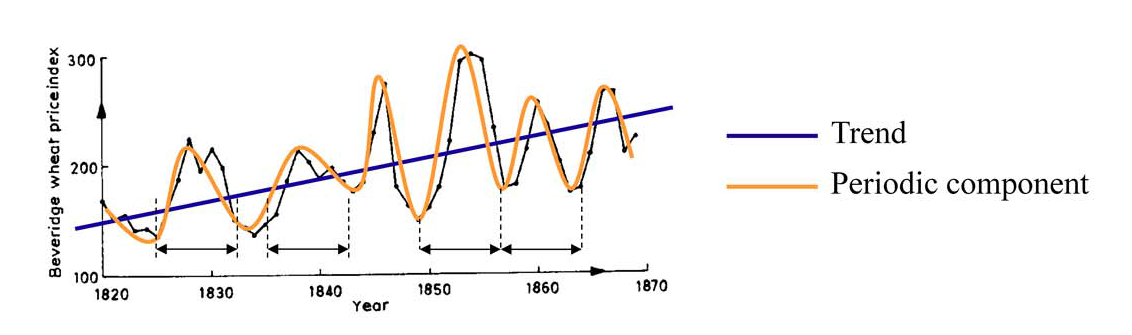
\includegraphics[width=0.9\linewidth]{images/time_series_example}
\caption{The Beveridge wheat price index is the average in nearly 50 places in various countries measured in successive years from 1500 to 1869. \protect\footnotemark}
\label{fig:time_series_example}
\end{figure}
\footnotetext{This time series can be downloaded from \url{http://www.york.ac.uk/depts/maths/data/ts/ts04.dat}}

\noindent According to Chatfield, most time series exhibit a variation at a fixed period of time (seasonality) such as for example the seasonal variation of temperature. Beyond this cycle, there exists either or both a long term change in the mean (trend) that can be linear, quadratic, and a periodic (cyclic) component. By definition, a signal is periodic of period $R$ if $x_{t+R}=x_t$ for all time instants $t$. In practice, this condition is not valid for real time series. In our work, we focus on the raw time series and do not try to extract global features from the time series.

Due to their complexity, other authors made the hypothesis of independency between the observations $x_{it}$. They consider time series as a static vector data (samples) and use classic machine learning algorithms \todo{[biblio time series static learning]}.


% Nous désignons par données temporelles des données numériques évoluant dans le temps, dites communément séries temporelles, ou des suites chronologiques de données symboliques dites séquences temporelles. Plus généralement, on désigne par données de séquences toute collection de données ordonnées selon un critère qui peut être sémantique, biologique, temporel ou autre ; c’est le cas, par exemple, des séquences de mots dans un texte ; on parle alors d’ordre syntaxique, de séquences d’acides aminés composant une chaîne d’ADN ou de peptides constituant une protéine.


%----------------------------------------------------------------------------
\section{Machine learning algorithms}

We are going to detail now a few number of machine learning algorithms used classically to solve classification or regression problems. Other algorithms are popular nowadays such as Deep neural network, Decision tree or Relevance vector machine. We focus on $k$-Nearest Neighbors ($k$-NN) and Support Vector Machine (SVM) because these algorithms are based on the comparison of samples (time series in our case) through a distance measure, notion detailed in the next chapters.

\subsection{Classification, regression}
The idea of Machine learning (also refer as Pattern learning or Pattern recognition) is to imitate with algorithms executed on computers, the ability of living beings to learn from examples. For example, to teach a child how to read letters, we show him during the training phase labeled examples of letters ('A', 'B', 'C', etc.) written in different styles and fonts. We don't give him a complete and analytic description of the topology of the characters but labeled examples. After the training phase (testing phase), we want the child to be able to recognize and to label correctly the letters that have been seen during the training, and also to generalize to new instances \cite{Dreyfus2006}. 

Let $\textbf{X}=\{\textbf{x}_i,y_i\}_{i=1}^n$ be a training set of $n$ samples $\textbf{x}_i$ (time series in our case) and $y_i$ their corresponding labels. The aim of Machine learning is to learn a relation (model) $f$ between the samples $\textbf{x}_i$ and their labels $y_i$ based on examples. This relationship can include static relationships, correlations, dynamic relationship, etc. After the training phase based on labeled examples $(\textbf{x}_i,y_i)$, the model $f$ has to be able to generalize on the testing phase, i.e., to give a correct prediction $y_j$ for new instances $\textbf{x}_j$ that haven't been seen during the training.

When $y_i$ are class labels (i.e., class 'A', 'B', 'C'), learning the model $f$ is a classification problem; when $y_i$ is a continuous value (i.e., the energy consumption in a building), learning $f$ is a regression problem. Both problems corresponds to supervised learning as $\textbf{x}_i$ and $y_i$ are known during the training phase \todo{[biblio supervisé]}. For both problems, when a part of the labels $y_i$ are known and an other part of $y_i$ is unknown during training, learning $f$ is a semi-supervised problem \todo{[biblio semi-supervisé]}. Note that when the labels $y_i$ are unknown, learning $f$ refers to a clustering problem (unsupervised learning) \todo{[biblio clustering]}. Our work focus on supervised learning (classification, regression).


\subsection{$k$-Nearest Neighbors ($k$-NN)}
%\begin{itemize}
%	\item Donner l'intuition
%	\item Formaliser le problème en tant que problème d'optimisation
%	\item Présenter les extensions (kNN pondéré), extension à la régression
%	\item Soulever le fait que la résolution du problème fait intervenir une notion de distance entre les individus (time series)	
%	\item Donner les arguments qui permettent de dire pourquoi utiliser un 1-NN permet de faire une évaluation de métriques (Ding)
%\end{itemize}

A simple approach to classify samples is to consider that "close" samples have a great probability to belong to the same class. Given a test sample $\textbf{x}_j$, one can decide that $\textbf{x}_j$ belong to the same class of its nearest neighbor in the training set. More generally, we can consider the $k$ nearest neighbors of $\textbf{x}_j$. The class $y_j$ of the test sample $\textbf{x}_j$ is assigned with a voting scheme among them, i.e., using the majority of the class of nearest neighbors. This algorithm is refer as the $k$-nearest neighbors algorithm ($k$-NN) \cite{Duda1973,Dreyfus2006}. Fig. \ref{fig:kNN_example} illustrates the concept for a neighborhood of $k=3$ and $k=5$.

\begin{figure}
\centering
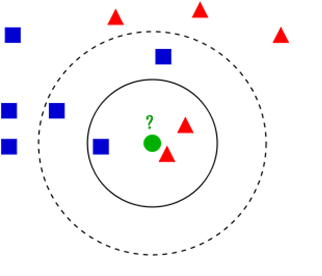
\includegraphics[width=0.4\linewidth]{images/kNN_example}
\caption{Example of $k$-NN classification. The test sample (green circle) is classified either to the first class (blue squares) or to the second class (red triangles). If $k = 3$ (solid line circle) it is assigned to the second class because there are 2 triangles and only 1 square inside the inner circle. If $k = 5$ (dashed line circle) it is assigned to the first class (3 squares vs. 2 triangles inside the outer circle).}
\label{fig:kNN_example}
\end{figure}

\noindent A key point in the $k$-NN algorithm is that the notion of "closeness" between samples is based on the computation of a metric \footnote{A clarification of the terms metric, distance, dissimilarity, etc. will be given in Chapter \ref{sec:Chapter_metrics}. For now, we refer all of them as metrics.}. Let $D$ be a metric. Usally, for static data, standard metrics are the Euclidean distance, the Minkowski distance or the Mahalanobis distance\footnote{A recall of these metrics will be in Chapter \ref{sec:Chapter_metrics}.}. Solving the 1-NN classification problem is equivalent to solve the optimization problem: \\
\noindent For a new sample $\textbf{x}_j$, $\forall i \in \{1...n\}$,
\begin{equation}
y_j = y_{i^*}
\end{equation}
where $i^*={\underset{i \in \{1...n\}}{\argmin}   D(\textbf{x}_i,\textbf{x}_j)}$.
\todo{Generalize for kNN}

The $k$-NN algorithm can be extended to estimate continous labels (regression problems). The procedure is similar. The label $y_j$ is defined as :
\begin{equation}
y_j = \sum_{i=1}^{k} y_{i}
\end{equation}
where $i$ corresponds to the index of the $k$-nearest neighbors\todo{[biblio regression kNN]}. There exists other variants of the $k$-NN algorithms: in a weighed $k$-NN, the approach consists in weighting each neighbors labels $y_{i}$ by a factor equal to the inverse of the distance $\frac{1}{D(\textbf{x}_i, \textbf{x}_j)}$ \todo{[biblio kNN pondéré]}; in a fuzzy $k$-NN, the idea is to assign memberships of samples $\textbf{x}_j$ to classes. The class membership is a function of the sample’s distance $D(\textbf{x}_i, \textbf{x}_j)$ from its $k$-NN training samples.\todo{[biblio fuzzy kNN]}.

Despite its simplicity, the $k$-NN algorithm presents many advantages and have been shown to be successful on time series classification problems \cite{Xi2006a,Ding2008}. One main advantage is that a 1-NN classifier can be used to evaluate and compare the efficacy of different metrics \cite{Ding2008}. First, the underlying metric is critical in the performance of the 1-NN classifier \cite{Tan2005b}. Thus, the accuracy of the 1-NN classifier directly reflects the effectiveness of the metric. Second, 1-NN classifier is easy to implement and doesn't need to learn any hyper-parameters, which make it straightforward for anyone to reproduce results. All of this advantages allows one who want to evaluate a benchmark of metrics. Other methods exists such as clustering with small data sets which are not statistically significant, or compare the compactness of the metric \todo{bilbio}. The 1-NN algorithm will be used in our experiments to compare the performances different metrics used for time series.

On the other hand, the $k$-NN algorithm presents some disavantages, mainly due to its computational complexity, both in space (storage of the training samples $\textbf{x}_i$) and time (search) \cite{Duda1973}. Suppose we have $n$ labelled training samples in $T$ dimensions, and find the closest neighbors to a test sample $\textbf{x}_j$ ($k = 1$). In the most simple approach, we look at each stored samples $\textbf{x}_i$ ($i=1...n$) one by one, calculate its metric to $\textbf{x}_i$ (D($\textbf{x}_i$,$\textbf{x}_j$)) and retain the index of the current closest one. For the standard Euclidean distance, each metric computation is $O(T)$ and thus the search is $O(Tn^2)$. Moreover, using standard metrics (such as the Euclidean distance) uses all the $T$ dimensions in its computation and thus assumes that all dimensions have the same effect on the metric. This assumption may be wrong and can impact the classification performances. Wrong classification due to presence of many irrelevant dimensions is refered as the curse of dimensionality. The importance of defining adapted metrics for time series will be discussed in Chapter \ref{sec:Chapter_metrics}.


% \textcolor{red}{Accuracy evaluation answers one of the most important questions about a similarity measure: why is this a good measure for describing the (dis)similarity between time series? Surprisingly, we found that accuracy evaluation is usually insufficient in existing literature: it has been either based on subjective evaluation, e.g., [4, 9], or using clustering with small data sets which are not statistically significant, e.g., [31, 40]. In this work, we use an objective evaluation method recently proposed [25]. The idea is to use a one nearest neighbor (1NN) classifier [17, 32] on la- belled data to evaluate the efficacy of the distance measure used. Specifically, each time series has a correct class label, and the classifier tries to predict the label as that of its nearest neighbor in the training set. There are several advantages with this approach. First, it is well known that the underlying distance metric is critical to the performance of 1NN classifier [32], hence, the accuracy of the 1NN classifier directly reflects the effectiveness of the similarity measure. Second, the 1NN classifier is straightforward to implement and is parameter free, which makes it easy for anyone to reproduce our results. Third, it has been proved that the error ratio of 1NN classifier is at most twice the Bayes error ratio [36]. Finally, we note that while there have been attempts to classify time series with decision trees, neural networks, Bayesian networks, supporting vector machines etc., the best published results (by a large margin) come from simple nearest neighbor methods [42]}

% Cons of the kNN
%Curse of Dimensionality
%* Distance usually relates to all the attributes and assumes all
%of them have the same effects on distance
%* The similarity metrics do not consider the relation of
%attributes which result in inaccurate distance and then impact
%on classification precision. Wrong classification due to
%presence of many irrelevant irrelevant attributes attributes is often termed as the
%curse of dimensionality
%* For example: Each instance is described by 20 attributes out
%of which only 2 are relevant in determining the classification
%of the target function. In this case, instances that have
%identical values for the 2 relevant attributes may
%nevertheless be distant from one another in the 20
%dimensional instance space
%(http://www.csee.umbc.edu/~tinoosh/cmpe650/slides/K_Nearest_Neighbor_Algorithm.pdf)


\subsection{Support Vector Machine (SVM)}
%\begin{itemize}
%	\item Présenter le principe général des SVM en commençant par l'intuition.
%	\item Forme primale: donner la formulation primale du problème d'optimisation
%	\item Forme duale: montrer commencer passer de la forme primal à la forme dual.
%	\item A partir de la forme duale, passer au kernel
%	\item Finir par la complexité du SVM en apprentissage ($o(N^3p)$) et en test (limités aux nombres de support vectors) et les interprétations des supports vectors.
%	\item Expliquer la modification du problème initiale avec une régularisation L1 sur le terme de régularisation et nous permet d'avoir une solution sparse (donner 1 cas où la solution sparse est meilleur).
%	\item Expliquer que dans le cadre de données non-balancées, il faut ajouter des termes pour rebalancer l'équation du SVM
%\end{itemize}

Support Vector Machine (SVM) is a state-of-the-art classication method
introduced in 1992 by Boser, Guyon, and Vapnik \cite{Boser1992,Cortes1995}. The SVM classifier have demonstrate high accuracy, ability to deal with high-dimensional data, good generalization properties and interpretation for various applications from recognizing handwritten digits, to face identification, text categorisation, bioinformatics and database marketing \cite{Campbell2011}. SVMs belong to the category of kernel methods, algorithms that depends on the data only through dot-products \cite{Schlkopf2013}.

As SVMs will be used in Chapter \ref{chap:formalization}, we first present an intuition of maximum margin concept. We give the primal formulation of the SVM optimization problem. Then, by transforming the latter formulation into its dual form, the kernel trick can be applied to learn non-linear classifiers. Finally, we detail how we can interpret the obtained coefficients and how SVMs can be extended for regression problems.

Note that this section doesn't aim to give an detailed comprehension of SVMs. It aims to give an overview of the mathematical key points interpretation and comprehension of the method and an interpretation and comprehension. For more informations, the reader can consult \cite{Schlkopf2013,Campbell2011,Cortes1995}.

\subsubsection{Intuition}
\todo[color=green]{Michèle: chiffre ou lettre pour la numérotation?}
Let consider a classification problem with 2 classes ($y_i= \pm 1$). The objective is to learn a hyperplan, whose equations are $\textbf{w}. \textbf{x} + b = 0$, that can separate samples of class +1 from the ones of class -1. When the problem is linearly separable such as in Fig. \ref{fig:Plusieurs_separatrice_lineaire}, there exists an infinite number of hyperplans. 

\begin{figure}[h!]
\centering
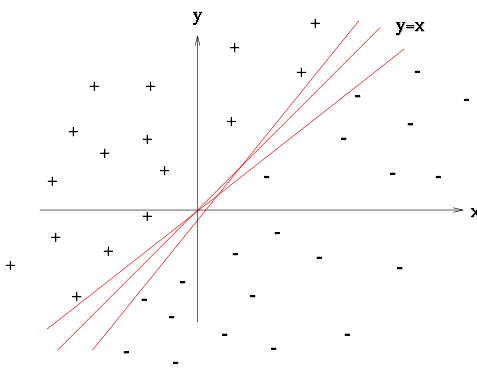
\includegraphics[width=0.4\linewidth]{images/Plusieurs_separatrice_lineaire}
\caption{Example of linear classifiers in a 2-dimensional plot. For a set of points of classes +1 and -1 that are linearly separable, there exists an infinite number of separating hyperplans corresponding to $\textbf{w}.\textbf{x} + b = 0.$}
\label{fig:Plusieurs_separatrice_lineaire}
\end{figure}

\noindent Vapnik \& al. \cite{Cortes1995} propose to choose the separating hyperplane that maximizes the margin, e.g. the hyperplane that leaves as much distance as possible between the hyperplane and the closest examples of each class, called the support vectors. This distance is equal to $\frac{1}{||\textbf{w}||_2}$. The hyperplanes passing through the support vectors of each class are refered as the canonical hyperplanes, and the region between the canonical hyperplanes is called the margin band (Fig. \ref{fig:Separatrice_lineaire_avec_marges}).

\begin{figure}[h!]
\centering
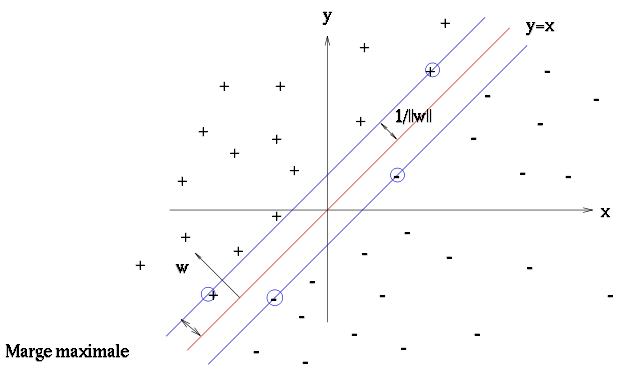
\includegraphics[width=0.6\linewidth]{images/Separatrice_lineaire_avec_marges}
\caption{The argument inside the decision function of a classifier is $\textbf{w}.\textbf{x} + b$. The separating hyperplane corresponding to $\textbf{w}.\textbf{x} + b = 0$ is shown as a line in this 2-dimensional plot. This hyperplane separates the two classes of data with points on one side labelled $y_i = +1$ ($\textbf{w}.\textbf{x} + b \geq 0$) and points on the other side labelled $y_i=-1$ ($\textbf{w}.\textbf{x} + b < 0$). Support vectors are circled in blue and lies on the hyperplans $\textbf{w}.\textbf{x} + b = +1$ and $\textbf{w}.\textbf{x} + b = -1$}
\label{fig:Separatrice_lineaire_avec_marges}
\end{figure}

% \missingfigure{Make a figure with many hyperplans. Put the one that maximize the hyperplan between the support vectors. Example of caption: }



\subsubsection{Primal formulation}
Finding $\textbf{w}$ and $b$ by maximizing the margin $\frac{1}{||\textbf{w}||_2}$ is equivalent to minimizing the norm of $\textbf{w}$ such that all samples from the training set are correctly classified:
	\begin{align}
		& \argmin_{\textbf{w},b} ||\textbf{w}||_2^2 \label{eq:objectiveSVM}\\
		& \textbf{s.t. } y_i(\textbf{w}.\textbf{x}_i+b) \geq 1 \label{eq:constraintsSVM}
	\end{align}
This is a constrained optimization problem in which we minimize an objective function (Eq. \ref{eq:objectiveSVM}) subject to constraints (Eq. \ref{eq:constraintsSVM}). This formulation is refered as the primal hard margin problem. Many real life datasets are subjected to noise and SVM can lead to poor generalization if it tries to fit to this noise, represented by the constraints in Eq. \ref{eq:constraintsSVM}. The effects of noise can be reduced by introducing slack variables $\xi_i \geq 0$ to relax the optimization problem:
	\begin{align}
	& \argmin_{\textbf{w},b}  
	\left( 
	\overbrace{\vphantom{\sum_{i=1}^n \xi_i}
		\frac{1}{2}||\textbf{w}||^2_2}^{Regularization}
	+ C \overbrace{\sum\limits_{i=1}^{n}\xi_i(\textbf{w}; b; x_i; y_i)}^{Loss} \right) 
	\label{eq:objectiveSVM2}\\
	& \textbf{s.t. } y_i(\textbf{w}.\textbf{x}_i+b) \geq 1 -\xi_i \label{eq:constraintsSVM2} \\
	&  \xi_i \geq 0 \label{eq:constraintsSVM20}
	\end{align}
\noindent where $C > 0$ is a penalty hyper-parameter. 
	
This formulation is refered as the primal soft margin problem. It is quadratic programming optimization problem subjected to constraints. Thus, it is a convex problem: any local solutions is a global solution. The objective function in Eq.~\ref{eq:objectiveSVM2} is made of two terms. The first one, the regularization term, penalize the complexity of the model and thus, controls the ability of the algorithm to generalize on new samples. The second one, the loss term, is an adaptation term to the data. The hyper-parameter $C$ is a trade-off between the regularization and the loss term. When $C$ tends to $+\infty$, the problem is equivalent to the primal hard margin problem. The hyper-parameter $C$ is learnt during the training phase. 

For SVM, the two common loss functions $\xi_i$ are max(1-$y_i \textbf{w}. \textbf{x}_i, 0)$ and max(1-$y_i \textbf{w}.\textbf{x}_i, 0)^2$. The former is referred to as L1-Loss and the latter is L2-Loss function. L2-loss function will penalize more slack variables $\xi_i$ during training. Theorically, it should lead to less error in training and poorer generalization in most of the case.

An other thing to specify is the type of regularizer. For SVM, the two common regularizer are $||\textbf{w}||_2$ and $||\textbf{w}||_2^2$. The former is referred to as L1-Regularizer while the latter is L2-Regularizer. L1-Regularizer is used to obtain sparser models than L2-Regularizer. Thus, it can be used for variable selection. L2-Regularizer allows to transform the primal formulation into a dual form.

\noindent From this, for a binary classification problem, to classify a new sample $\textbf{x}_j$, the decision function is:
\begin{equation}
	f(\textbf{x}_j) = sign(\textbf{w}. \textbf{x}_j + b)
\end{equation}

\subsubsection{Dual formulation}
From the primal formulation, using a L2-Regularizer, it is possible to have an equivalent dual form. This latter formulation allows samples $\textbf{x}_i$ to appear in the optimization problem through dot-products only. Thanks to that, a Kernel trick can be applied to extend the methods to learn non-linear classifiers.

First, to simplify the calculation development, let consider the hard margin formulation in Eq. \ref{eq:objectiveSVM2}, \ref{eq:constraintsSVM2} and \ref{eq:constraintsSVM20} with a L1-Loss function. As a constrained optimization problem, the formulation is equivalent to the minimization of a Lagrange function, consisting of the sum of the objective function and the $n$ constraints multiplied by their respective Lagrange multipliers: 
\begin{align}
	& \argmax_{\alpha} \left( L(\textbf{w},b) = \frac{1}{2}(\textbf{w}.\textbf{w})-\sum\limits_{i=1}^{n}\alpha_i(y_i(\textbf{w}.\textbf{x}_i+b)-1) \right) \label{eq:Lagrange} \\
	& \textbf{s.t. KKT } \forall i = 1...n: \\
	& \alpha_i \geq 0 \label{KKT1}\\
	& y_i(\textbf{w}.\textbf{x}_i+b)-1 \geq 0 \label{KKT2}\\
	& \alpha_i (y_i(\textbf{w}.\textbf{x}_i+b)-1) = 0 \label{KKT3}
\end{align}
\noindent where $\alpha_i \geq 0$ are the Lagrange multipliers. Eq. \ref{KKT1}, \ref{KKT2} and \ref{KKT3} are called in optimization theory the Karush-Kuhn-Tucker (KKT) conditions. It corresponds to the set of conditions which must be satisfied at the optimum of a constrained optimization problem. The KKT conditions will play an important role in the interpretation of SVM in Section \ref{subsec:interpretation}. 

\noindent At the minimum, we can take the derivatives with respect to $b$ and $\textbf{w}$ and set them to zero:
\begin{align*}
\frac{\partial L}{\partial b} &= \sum\limits_{i=1}^{n}\alpha_i y_i = 0 \\
\frac{\partial L}{\partial \textbf{w}} &= \textbf{w}-\sum\limits_{i=1}^{n}\alpha_i y_i \textbf{x}_i = 0
\end{align*}
\noindent that leads to:
\begin{align}
&\sum\limits_{i=1}^{n}\alpha_i y_i = 0 \\
& \textbf{w} = \sum\limits_{i=1}^{n}\alpha_i y_i \textbf{x}_i
\end{align}

\noindent By substituing $\textbf{w}$ into $L(\textbf{w},b)$ in Eq. \ref{eq:Lagrange}, we obtain the dual formulation (\textit{Wolfe dual}):
\begin{align}
	& \argmax_\alpha \left( 
	\sum\limits_{i=1}^{n} \alpha_i - \frac{1}{2} \sum\limits_{i,j=1}^{n} \alpha_i \alpha_j y_i y_j (\textbf{x}_i . \textbf{x}_j) 
	\right) 
	\label{eq:dualSVM}\\
	& \textbf{s.t. } \sum\limits_{i=1}^{n}\alpha_i y_i = 0 \label{constraintdual1}\\
	& \alpha_i \geq 0 \label{constraintdual2}
\end{align}
where $\alpha$ is the vector of corresponding $\alpha_i$: $\alpha = [\alpha_1, ..., \alpha_n]'$. The dual objective in \ref{eq:dualSVM} is quadratic in the parameters $\alpha_i$. Adding the constraints in Eq. \ref{constraintdual1} and \ref{constraintdual2}, it is a constrained quadratic programming optimization problem (QP). Note that while the primal formulation is minimization, the equivalent dual formulation is maximization. It can be shown that the objective functions of both formulations reach the same value when the solution is found \cite{Campbell2011}. In the same spirit, considering the soft margin primal problem, it can be shown that it leads to the following formulation \cite{Campbell2011}:
\begin{align}
& \argmax_\alpha 
\left( 
\sum\limits_{i=1}^{n} \alpha_i - \frac{1}{2} \sum\limits_{i,j=1}^{n} \alpha_i \alpha_j y_i y_j (\textbf{x}_i . \textbf{x}_j) 
\right) 
\label{eq:dualSVM2}\\
& \textbf{s.t. } \sum\limits_{i=1}^{n}\alpha_i y_i = 0 \label{constraintdual3}\\
& 0 \leq \alpha_i \leq C  \label{constraintdual4}
\end{align}
\noindent The only difference between the hard margin and soft margin formulation in its dual form is that the Lagrange multipliers $\alpha_i$ are upper bounded by the trade-off $C$ in the soft margin formulation. The constraints in Eq. \ref{constraintdual4} are called the Box constraints \cite{Campbell2011}. From the optimal value of $\alpha_i$, denoted $\alpha_i^*$, it is possible to compute the weight vector $\textbf{w}^*$ and the bias $b^*$ at the optimality:
\begin{align}
	\textbf{w}^* & = \sum\limits_{i=1}^{n}\alpha_i^* y_i \textbf{x}_i \\
	b^* & = \sum\limits_{i=1}^{n} (\textbf{w}.\textbf{x}_i - y_i)
\end{align}
At the optimality point, only a few number of datapoints have $\alpha_i^* > 0$ as shown as in Fig. \ref{fig:SVM_SV}. These samples are the vector supports. All other datapoints have $\alpha_i^*=0$, and the decision function is independent of them. Thus, the representation is sparse. 

\noindent From this, to classify a new sample $\textbf{x}_j$, the decision function for a binary classification problem is:
\begin{equation}
	f(\textbf{x}_j) = sign(\sum\limits_{i=1}^{n} \alpha_i^*y_i(\textbf{x}_i.\textbf{x}_j) + b^*) \label{decisionDual}
\end{equation} 

\begin{figure}[h!]
\centering
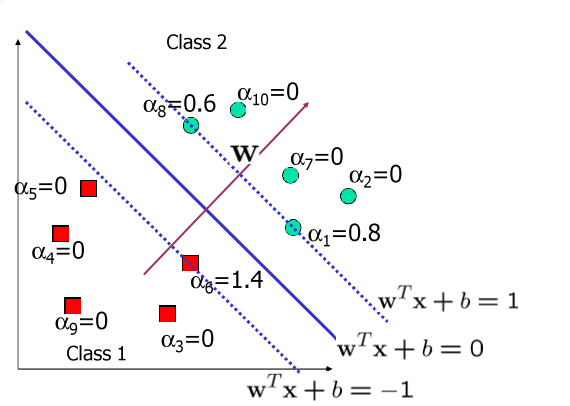
\includegraphics[width=0.6\linewidth]{images/SVM_SV}
\caption{Obtained hyperplan after a dual resolution (full blue line). The 2 canonical hyperplans (dash blue line) contains the support vectors whose $\alpha_i > 0$. Other points have their $\alpha_i = 0$ and the equation of the hyperplan is only affected by the support vectors.}
\label{fig:SVM_SV}
\end{figure}


\subsubsection{Kernel trick}
The concept of Kernels was introduced by Aizerman \& Al in 1964 to design potential functions in the context of pattern recognition \cite{Aizerman1964}. The idea was re-introduced in 1992 by Boser \& al. for Support Vector Machine (SVM) and has been received a great number of improvments and extensions to symbolic objects such as text or graphs \cite{Boser1992}.

One theorical interesting property of SVM if that it has been shown that the generalization error bound does not depend on the dimensionality $T$ of the space \cite{Schlkopf2013}. From the dual objective in Eq. \ref{eq:dualSVM}, we note that the samples $\textbf{x}_i$ are only involves in a dot-product. Therefore, we can map these samples $\textbf{x}_i$ into a higher dimensional hyperspace, called the feature space, through the replacement:
\begin{equation}
	(\textbf{x}_i . \textbf{x}_j) \rightarrow \Phi(\textbf{x}_i) . \Phi(\textbf{x}_j) 
\end{equation}
\noindent where $\Phi$ is the mapping function. The intuition behind is that in many datasets, it is not possible to find a hyperplan that can separate the two classes in the input space. The problem is not linearly separable. However, by applying a transformation $\Phi$, data might become linearly separable in a higher dimensional space (feature space). Fig. \ref{fig:SVM_nonlinear} illustrates the idea: in the original 2-dimensional space (left), the two classes can't be separated by a line. However, with a third dimension such that the $+1$ labelled points are moved forward and the $-1$ labelled moved back the two classes become separable.

In most of the case, the mapping function $\Phi$ does not need to be known since it will be defined by the choice of a Kernel: $K(\textbf{x}_i,\textbf{x}_j)= \Phi(\textbf{x}_i) . \Phi(\textbf{x}_j)$. We call Gram matrix $G$, the matrix containing all $K(\textbf{x}_i,\textbf{x}_j)$:
\begin{equation*}
	G = (K(\textbf{x}_i,\textbf{x}_j))_{1 \leq i,j \leq n} = 
	\begin{pmatrix}
	K(\textbf{x}_1,\textbf{x}_1) & ... & K(\textbf{x}_1,\textbf{x}_n) \\
	... & & ... \\
	K(\textbf{x}_n,\textbf{x}_1) & ... & K(\textbf{x}_n,\textbf{x}_n) 
	\end{pmatrix}
\end{equation*}

\noindent Defining a kernel has to follow rules. One of them is that it has to define a proper inner product in the feature space. Mathematically, the Gram matrix has to be semi-definite positive (Mercer's theorem) \cite{Schlkopf2013}. These restricted feature spaces, containing an inner product are called Hilbert space.


\begin{figure}[h!]
\centering
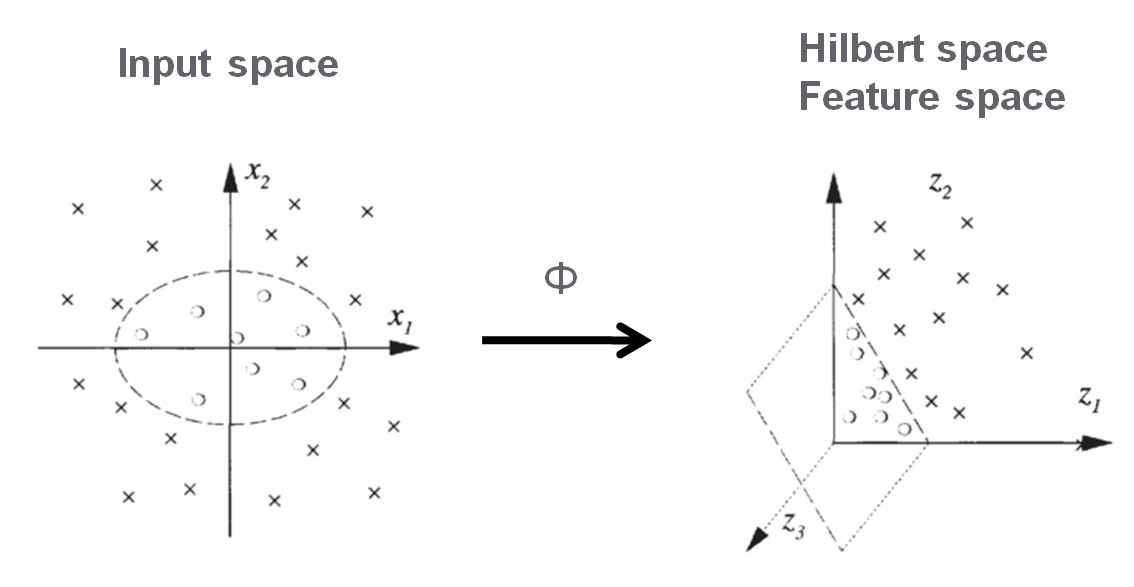
\includegraphics[width=0.9\linewidth]{images/SVM_nonlinear}
\caption{Left: in two dimensions these two classes of data are mixed together, and it is not possible to separate them by a line: the data is not linearly separable. Right: using a Gaussian kernel, these two classes of data (cross and circle) become separable by a hyperplane in feature space, which maps to the nonlinear boundary shown, back in input space.}
\label{fig:SVM_nonlinear}
\end{figure}

Many kernels have been proposed in the litterature such as the polynomial, sigmoid, exponential or wavelett Kernels \cite{Schlkopf2013}. The most popular ones that we will use in our work are respectively the Linear and the Gaussian (or Radial Basis Function (RBF)) Kernels:
\begin{align}
	& K(\textbf{x}_i,\textbf{x}_j)= \textbf{x}_i . \textbf{x}_j \\
	& K(\textbf{x}_i,\textbf{x}_j)
	= \exp(-\frac{||\textbf{x}_j-\textbf{x}_i||_2^2}{2\sigma^2})
	= \exp(-\gamma.||\textbf{x}_j-\textbf{x}_i||_2^2)
\end{align}
where $\gamma = \frac{1}{2\sigma^2}$ is the parameter of the Gaussian Kernel and $||\textbf{x}_j-\textbf{x}_i||_2$ is the Euclidean distance between $\textbf{x}_i$ and $\textbf{x}_j$. Note that the Linear kernel is an identity transformation. In practice, for large scale problem (when $T$ is high), using a Linear Kernel is sufficient  \cite{Fan2008}.

The Gaussian Kernel computed between a sample $\textbf{x}_j$ with a support vector $\textbf{x}_i$ is an exponentially decaying function in the input feature space. The maximum value of the Kernel ($K(\textbf{x}_i,\textbf{x}_j)$=1) is attained at the support vector (when $\textbf{x}_i=\textbf{x}_j$). Then, the value of the Kernel decreases uniformly in all directions around the support vector, with distance and ranges between zero and one. It can thus be interpreted as a similarity measure. Geometrically speaking, it leads to hyper-spherical contours of the kernel function as shown in Fig. \ref{fig:Kernel_Gaussian} \footnote{\url{https://www.quora.com/Support-Vector-Machines/What-is-the-intuition-behind-Gaussian-kernel-in-SVM}}. The parameter $\gamma$ controls the decreasing speed of the sphere. \todo{reformuler pour le gamma}. In pratice, this parameter is learnt during the training phase.


\todo{refaire la figure}
\begin{figure}[h!]
\centering
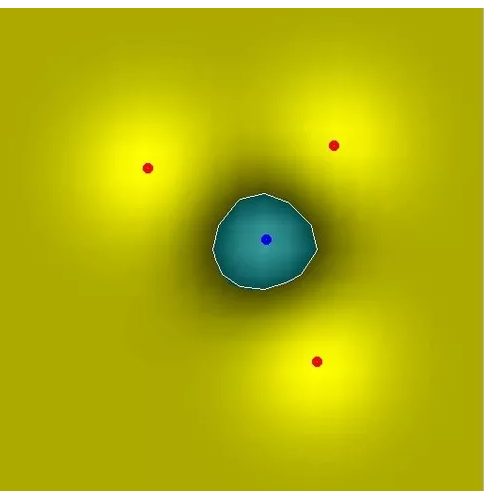
\includegraphics[width=0.4\linewidth]{images/Kernel_Gaussian}
\caption{Illustration of the Gaussian Kernel in the input space.}
\label{fig:Kernel_Gaussian}
\end{figure}


By applying the Kernel trick to the soft margin formulation in Eq. \ref{eq:dualSVM2}, \ref{constraintdual3} and \ref{constraintdual4}, the following optimization problem allows to learn non-linear classifiers:
\begin{align}
	& \argmax_\alpha \left( 
	\sum\limits_{i=1}^{n} \alpha_i - \frac{1}{2} \sum\limits_{i=1}^{n} \sum\limits_{j=1}^{n} \alpha_i \alpha_j y_i y_j K(\textbf{x}_i . \textbf{x}_j) 
	\right) 
	\label{eq:dualSVM2kernel}\\
	& \textbf{s.t. } \sum\limits_{i=1}^{n}\alpha_i y_i = 0 \label{constraintdual3kernel}\\
	& 0 \leq \alpha_i \leq C  \label{constraintdual4kernel}
\end{align}

\noindent and the decision function $f$ becomes:
\begin{equation}
f(\textbf{x}_j) = sign(\sum\limits_{i=1}^{n} \alpha_i^*y_i K(\textbf{x}_i.\textbf{x}_j) + b^*) \label{decisionDualKernel}
\end{equation} 
\noindent Note that in this case, we can't recover the weight vector $\textbf{w}^*$.
Let $n_{SV}$ be the number of support vectors ($n_{SV} \leq n$). To recover $b^*$, we recall that for support vectors $\textbf{x}_i$:
\begin{equation}
	y_j \left( \sum\limits_{i=1}^{n_{SV}} \alpha_i^* y_i K(\textbf{x}_i,\textbf{x}_j) + b^* \right) = 1
\end{equation}
From this, we can solve $b^*$ using an arbitrarily chosen support vector $\textbf{x}_i$:
\begin{equation}
	b^* = \frac{1}{y_j} - \sum\limits_{i=1}^{n_{SV}} \alpha_i^* y_i K(\textbf{x}_i,\textbf{x}_j)
\end{equation}

\subsubsection{Complexity and interpretation}
\label{subsec:interpretation}
%\begin{itemize}
%	\item interpretation dans le primal: vecteur w et b
%	\item interpretation dans le dual
%	\item interpretation
%\end{itemize}

\noindent \textbf{Complexity} \\
As the objective is to provide an algorithm for both small and large datasets, let us examine the complexity of SVMs, both in the resolution of the optimization problem (primal and dual) and in the computation of the Gram matrix $G$.
\todo[inline]{Finir la complexité}

\noindent \textbf{Interpretation in the primal} \\
In the primal, the weight vector $\textbf{w} = [w_1, \ldots, w_T]'$ contains as many elements as there are variables in the dataset, i.e., $\textbf{w} \in \mathbb{R}^T$. The magnitude of each element in $\textbf{w}$ denotes the importance of the corresponding variable for the classification problem. If the element of $\textbf{w}$ for some variable is 0, these variables are not important for the classification problem.

In order to visualize the above interpretation of the weight vector $\textbf{w}$, let us examine several hyperplanes $\textbf{w}.\textbf{x}+b=0$ shown in Fig. \ref*{fig:Weight_interpretation}. Figure (a) shows a hyperplane where elements of $\textbf{w}$ are the same for both variables $\textbf{x}_1$ and $\textbf{x}_2$. The interpretation is that both variables contribute equally for classification of objects into positive and negative. Figure (b) shows a hyperplane where the element of w for $\textbf{x}_1$ is 1, while that for $\textbf{x}_2$ is 0. This is interpreted as that $\textbf{x}_1$ is important but $\textbf{x}_2$ is not. An opposite example is shown in figure (c) where $\textbf{x}_2$ is considered to be important but $\textbf{x}_1$ is not. Finally, figure (d) provides a 3-dimensional example where an element of w for $\textbf{x}_3$ is 0 and all other elements are equal to 1. The interpretation is that $\textbf{x}_1$ and $\textbf{x}_2$ are important but $\textbf{x}_3$ is not.

\begin{figure}[h!]
	\centering
	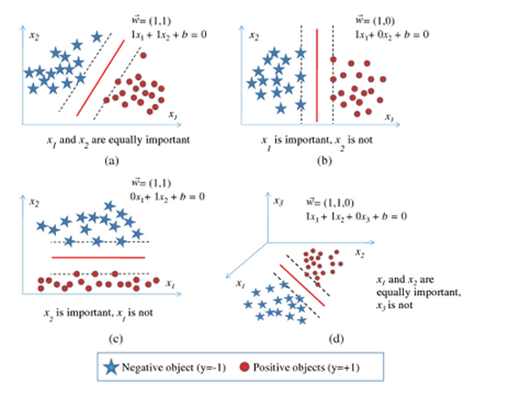
\includegraphics[width=0.7\linewidth]{Weight_interpretation}
	\caption{Example of several SVMs and how to interpret the weight vector $\textbf{w}$}
	\label{fig:Weight_interpretation}
\end{figure}

Another way to interpret how much a variable contributes in the vector $\textbf{w}$ is to express the contribution in percentage. To do that, if the variables $\textbf{X}_j$ are normalized before learning the SVM model, they evolves in the same range. Thus, the ratio $\frac{||w_j||_2}{||\textbf{w}||_2}*100$ defines the percentage of contribution for each variable $\textbf{X}_j$ in the SVM model.

Geometrically, the vector $\textbf{w}$ represents the direction of the hyperplan (Fig. \ref{fig:SVM_interpretation}). The bias $b$ is equal to the distance of the hyperplan to the origin point $\textbf{x}=\textbf{0}$\footnote{$\textbf{0}$ stands for the null vector: $\textbf{0} = [0, \ldots ,0]^T$}. The orthogonale projection of a sample $\textbf{x}_i$ on the direction $\textbf{w}$ is $P_\textbf{w}(\textbf{x}_i) = \textbf{w}.\textbf{x}_i$. In the soft margin problem, the slack variables $\xi_i$ of the samples $\textbf{x}_i$ that lies within the two canonical hyperplan are equal to zero. Outside of these canonical hyperplans, the slack variables $\xi_i > 0$ are equal to the distance to the hyperplan.


\begin{figure}[h!]
	\centering
	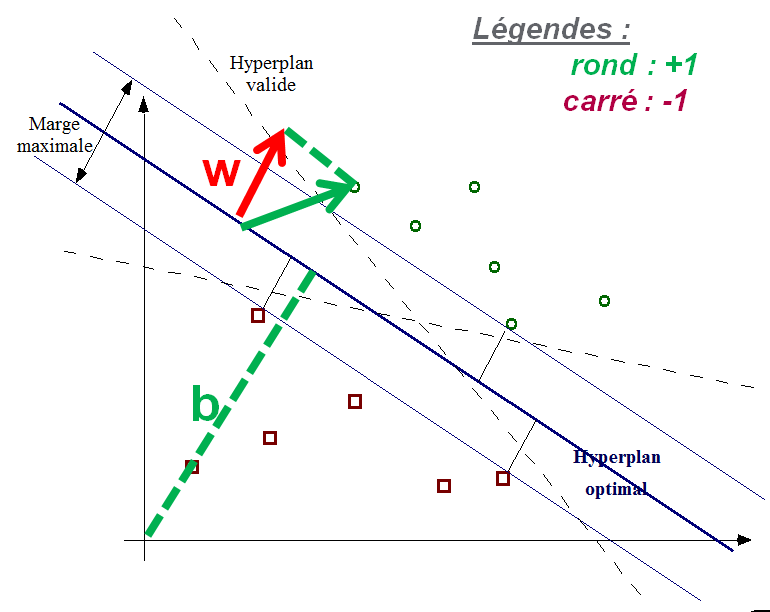
\includegraphics[width=0.5\linewidth]{images/SVM_interpretation}
	\caption{}
	\label{fig:SVM_interpretation}
\end{figure}


\noindent \textbf{Interpretation in the dual} \\
As a constrained optimization, the dual form satisfies the
Karush-Kuhn-Tucker (KKT) conditions (Eq. \ref{KKT1}, \ref{KKT2} and \ref{KKT3}). We recall Eq. \ref{KKT3})
\begin{equation*}
	\alpha_i (y_i(\textbf{w}.\textbf{x}_i+b)-1) = 0
\end{equation*}
From this, for every datapoint, either $\alpha_i^* = 0$ or $y_i(\textbf{w}.\textbf{x}_i+b) = 1$. Any datapoint with $\alpha_i^* = 0$ do not appear in the sum of the decision function $f$ in Eq. \ref{decisionDual} or \ref{decisionDualKernel}. Hence, they play no role in the prediction of new samples $\textbf{x}_j$. The others ($\alpha_i^* > 0$) corresponds to the support vector. Looking at the distribution of $\alpha_i^*$ allows also to have either a better understanding of the datasets, or either to detect outliers. The higher is the coefficient $\alpha_i^*$ for a sample $\textbf{x}_i$, the more the sample $\textbf{x}_i$ impacts on the decision function $f$. However, unusual high value of $\alpha_i^*$ among the samples can lead to two interpretations: either this point is a critical point to the decision, either this point is an outlier. By constraining $\alpha_i^*$ to be inferior to $C$ (Box constraints) in the soft margin problem, the effect of outliers can be reduced and controlled. 




\subsubsection{Extensions of SVM}
SVM has received many interests in recent years. Many extensions has been developped such as $\nu$-SVM, asymetric soft margin SVM or multiclass SVM \todo{Biblio}. One interesting extension is the extension of Support Vector Machine to regression problems, also called Support Vector Regression (SVR). The objective is to find a linear regression model $f(\textbf{x})=\textbf{w}.\textbf{x}+b$. To preserve the property of sparsiness, the idea is to consider an $\epsilon$-insensitive error function. It gives zero error if the absolute difference between
the prediction $f(\textbf{x}_i)$ and the target $y_i$ is less than $\epsilon$ where $\epsilon > 0$ penalize samples that are outside of a $\epsilon$-tube as shown as in Fig. \ref{fig:SVR_tube}.

\begin{figure}[h!]
\centering
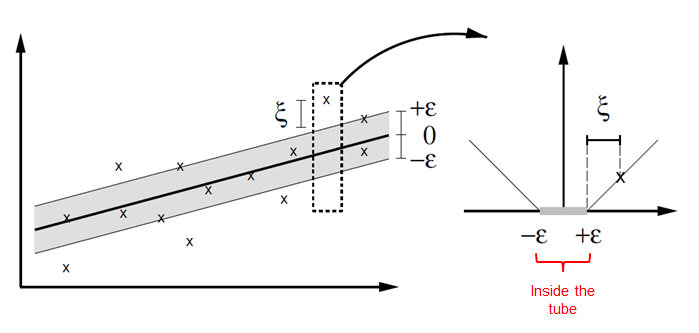
\includegraphics[width=0.9\linewidth]{images/SVR_tube}
\caption{Illustration of SVM regression (left), showing the regression curve with the $\epsilon$-insensitive "tube" (right). Samples $\textbf{x}_i$ above the $\epsilon$-tube have $\xi_1 > 0$ and $\xi_1 = 0$, points below the $\epsilon$-tube have $\xi_2 = 0$ and $\xi_2 > 0$, and points inside the $\epsilon$-tube have $\xi = 0$.}
\label{fig:SVR_tube}
\end{figure}

\noindent An example of $\epsilon$-insensitive error function $E_{\epsilon}$ is given by,
\begin{equation}
E_{\epsilon} (f(\textbf{x}_i)-y_i) =
\left\lbrace
\begin{array}{lll}
0  								& \mbox{if} 		& |f(\textbf{x}_i)-y_i| < \epsilon\\
|f(\textbf{x}_i)-y_i|-\epsilon 	& \mbox{otherwise}  & 
\end{array}\right.
\end{equation}


\noindent The soft margin optimization problem in its primal form is formalized as:
	\begin{align}
		& \argmin_{\textbf{w},b}  \left( 
		\overbrace{\vphantom{\sum_{i=1}^n \xi_i}
			\frac{1}{2}||\textbf{w}||^2_2}^{Regularization}
		+ C \overbrace{\sum\limits_{i=1}^{n}(\xi_{i_1}+\xi_{i_2})}^{Loss}
		\right) 
		\label{eq:objectiveSVR}\\
		& \textbf{s.t. } \forall i=1 \ldots n:\\
		& y_i-(\textbf{w}.\textbf{x}_i+b) \geq \epsilon -\xi_{i_1} \\
		& (\textbf{w}.\textbf{x}_i+b)-y_i \geq \epsilon -\xi_{i_2} \\
		&  \xi_{i_1} \geq 0 \\
		&  \xi_{i_2} \geq 0 \\
	\end{align}

\noindent The slacks variables are divided into 2 slacks variables, one for samples above the decision function $f$ ($\xi_{i_1}$), and one for samples under the decision function $f$ ($\xi_{i_2}$). As for SVM, it is possible to have a dual formulation:
	\begin{align}
		& \argmax_{\alpha} 
		\left( 
		\sum\limits_{i=1}^{n} y_i(\alpha_{i_1}-\alpha_{i_2})
		-\frac{1}{2} \sum\limits_{i=1}^{n} \sum\limits_{j=1}^{n} (\alpha_{i_1}-\alpha_{i_2})(\alpha_{j_1}-\alpha_{j_2}) (\textbf{x}_i.\textbf{x}_j)
		\right) \\ 
		& \textbf{s.t. } \forall i=1 \ldots n:\\
		& \sum\limits_{i=1}^{n} \alpha_{i_1} = \sum\limits_{i=1}^{n} \alpha_{i_2} \\
		& 0 \leq \alpha_{i_1} \leq C \\
		& 0 \leq \alpha_{i_2} \leq C
	\end{align}
\noindent As in SVM, we obtain three possible decision functions for a new sample $\textbf{x}_j$, respectively in its primal, dual, and non-linear form:
\begin{align}
	& f(\textbf{x}_j) = \textbf{w}.\textbf{x}_j+b \\ 
	& f(\textbf{x}_j) = \sum\limits_{i=1}^{n} (\alpha_{i_1}^*-\alpha_{i_2}^*)(\textbf{x}_i.\textbf{x}_j) + b \\	
	& f(\textbf{x}_j) = \sum\limits_{i=1}^{n} (\alpha_{i_1}^*-\alpha_{i_2}^*)K(\textbf{x}_i.\textbf{x}_j) + b
\end{align}	
More informations about the calculation develpment can be found in \cite{Bishop2006}.
\subsection{Other classification algorithms}
\todo[inline]{Partie non encore rédigée. A faire à la fin.}
\begin{itemize}
	\item S'intéresser au Deep neural network (à la mode en ce moment)
	\item RVM, Decision Tree, 
	\item Ne pas trop développer
	\item Dans notre cas, on ne s'intéressera pas à ce type d'algorithmes (type deep learning) car il ne repose pas sur une notion de distance et les features qui sont trouvés ne sont pas interprétables
\end{itemize}




%----------------------------------------------------------------------------
\section{Learning protocol}
\subsection{Supervised learning framework}
%\begin{itemize}
%	\item Learning framework (train, validation, test): la plupart des algorithmes requiert l'optimisation d'un hyper-paramètre. Le jeu de train permet d'apprendre les meilleurs hyper-paramètres.
%	\item Cross-validation (pourquoi on fait de la cross-validation, comment on la fait (Faire un schéma))
%\end{itemize}	

A key objective of learning algorithms is to build models $f$ with good generalization capability, i.e., models $f$ that correctly predict the class labels $y_j$ of new unknown samples $\textbf{x}_j$. Fig. \ref{fig:LearningFramework} shows a general approach for solving machine learning problems. First, a training set $X=\{(\textbf{x}_i,y_i)\}_{i=1}^n$ consisting of samples $\textbf{x}_i$ whose labels $y_i$ are known is provided. The training set is used to build the supervised model $f$. Then, the model is applied to the test set $X_T=\{(\textbf{x}_j,y_j)\}_{j=1}^m$, which consists of samples $\textbf{x}_j$ with unknown labels $y_j$. The test is used to evaluate the performance of the learnt model. 

\begin{figure}[h!]
\centering
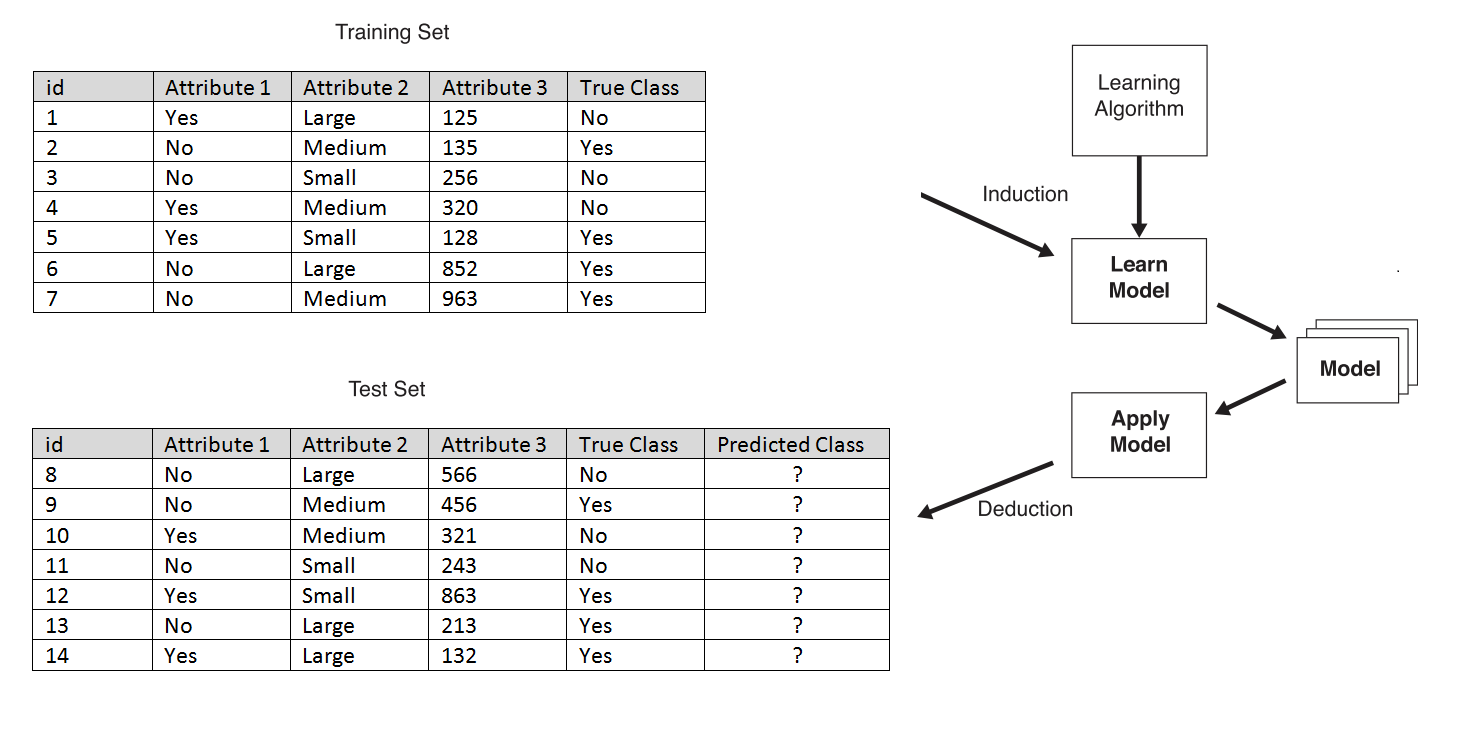
\includegraphics[width=0.7\linewidth]{images/LearningFramework}
\caption{General framework for building a supervised (classification/regression) model.}
\label{fig:LearningFramework}
\end{figure}

The errors committed by a classification or regression model are divided into two types: training errors and generalization errors (testing error). Training error is the number of misclassification errors in classification (Root Mean Square Error or other error measures in regression) committed on training samples $\textbf{x}_i$, whereas generalization error is the expected error of the model $f$ on unseen samples $\textbf{x}_j$. A good supervised model $f$ must not only fit the training data $X$ well, it must also accurately classify records it has never seen before $X_T$. In other words, a good model $f$ must have low training error as well as low generalization error. This is important because a model that fits the training data too well can have a poorer generalization error than a model with a higher training error. Such a situation is known as model overfitting (Fig. \ref{fig:Overfitting}).

\begin{figure}[h!]
\centering
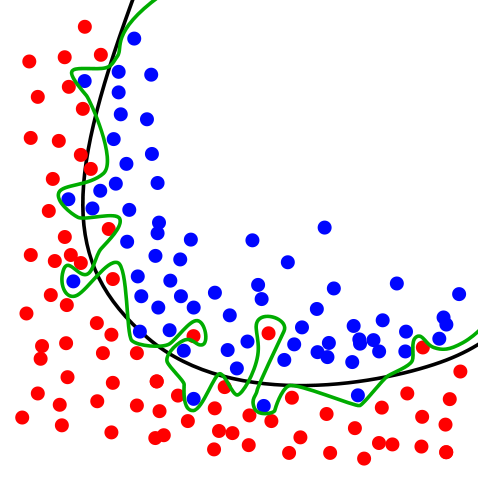
\includegraphics[width=0.4\linewidth]{images/Overfitting}
\caption{An example of overfitting for a classification problem. The objective is to separate blue points from red points. Black line shows a separator $f_1$ with low complexity where as green line illustrates a model $f_2$ with high compelexity. On training examples (blue and red points), the model $f_2$ separates all the classes perfectly but may lead to poor generalization on new unseen examples. }
\label{fig:Overfitting}
\end{figure}

In most cases, learning algorithms requires to tune some hyper-parameters. For that, the training set can be divided into 2 sets: a learning and a validation set. Suppose we have two hyper-parameters to tune: $C$ and $\gamma$. We make a grid search for each combination of the hyper-parameters, that is in this case a 2-dimensional grid (Fig. \ref{fig:GridSearch}). For each combination (a cell of the grid), the model is learnt on the learning set and evaluated on the validation set. At the end, the model with the lowest error on the validation set is retained. This process is refered as the model selection. 

\begin{figure}[h!]
\centering
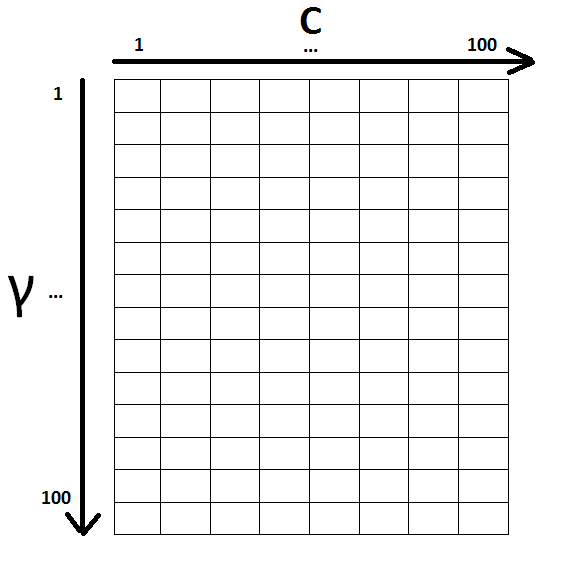
\includegraphics[width=0.4\linewidth]{images/GridSearch}
\caption{Example of a 2 dimensional grid search for parameters $C$ and $\gamma$. It defines a grid where each cell of the grid contains a combination ($C$, $\gamma$). Each combination is used to learn the model and is evaluated on the validation set.}
\label{fig:GridSearch}
\end{figure}

An alternative is cross-validation with $v$ folds, illustrated in Fig. \ref{fig:Cross_validation}. In this approach, we partition the training data into $v$ equal-sized subsets. The objective is to evaluate the error for each combination of hyper-parameters. For each run, one fold is chosen for validation, while the $v-1$ rest folds are used as the learning set. We repeat the process for each fold, thus $v$ times. Each fold gives one validation error and thus we obtain $v$ errors. The total error for the current combination of hyper-parameters is obtained by summing up the errors for all $v$ folds. When $v=n$, the size of training set, this approach is called leave-one-out. Each test set contains only one sample. The advantage is much data are used as possible for training. Moreover, the test sets are exclusive and they cover the entire data set. The drawback is that it is computationally expensive to repeat the procedure $n$ times. Furthermore, since each test set contains only one record, the variance of the estimated performance metric is usally high. This procedure is often used when $n$, the size training set, is small.

\begin{figure}[h!]
	\centering
	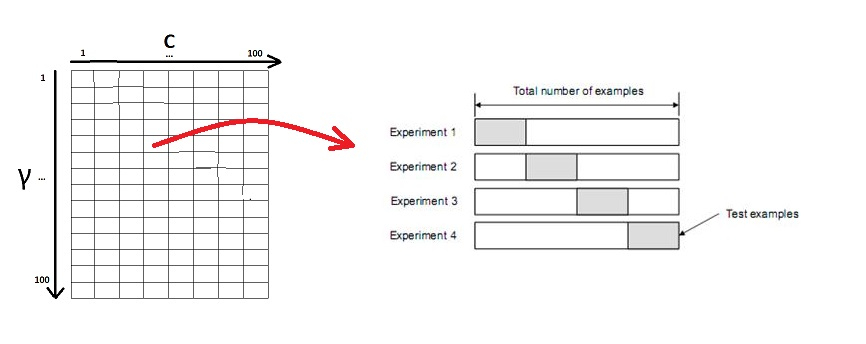
\includegraphics[width=\linewidth]{Cross_validation2}
	\caption{$v$-fold Cross-validation for one combination of parameters. For each of $v$ experiments, use $v-1$ folds for training and a different fold for Testing, then the training error for this combination of parameter is the mean of all testing errors. This procedure is illustrated for $v=4$.}
	\label{fig:Cross_validation}
\end{figure}

\noindent There exists other methods such as subsampling or bootstraps \cite{Duda1973,Dreyfus2006}. We use cross-validation in our experiments.

\subsection{Model evaluation}
\begin{itemize}
	\item Classification Error et test de significativité
	\item Regression Error
\end{itemize}


\subsubsection{Classification}
%This section reviews a statistical test for determining whether one learning learning algorithm outperforms another on a particular learning task.
%
%The accuracy or error rate computed from the test set can also be used to compare the relative performance of different classifiers on the same domain. Note that in order to do this, the class labels of the test records must be known.
%
%
%To apply the following test, we divide our available sample of data S, into a training set R and a test set T. We train algorithm A and B on the training set yielding classifiers $f_A$ and $f_B$. We then test these classifiers on the test set. For each example $x \in T$, we record how it was classified and construct the following contingency table:
%\begin{figure}[h] 
%	\centering
%	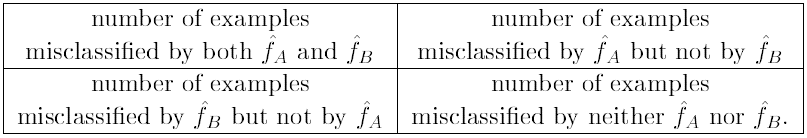
\includegraphics[width=0.7\linewidth]{ContingencyTable}
%	\caption{Contingency table}
%	\label{fig:ContingencyTable}
%\end{figure}
%
%\noindent We will use the notation
%\begin{figure}[h]
%	\centering
%	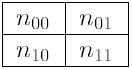
\includegraphics[width=0.1\linewidth]{ContingencyTable_notation}
%	\caption{Notation for the contingency table}
%	\label{fig:ContingencyTable_notation}
%\end{figure}
%
%where $n=n_{00}+n_{01}+n_{10}+n_{11}$ is the total number of examples in the test set T.
%
%
%A simple statistical test suggested in Dietterich \& Al. in 1997 is based on measuring the difference between the error rate of algorithm A and the error rate of algorithm B. Specifically, let $n$ be the number of test examples, $p_A = \frac{(n_{00}+n_{01}}{n})$ the proportion of test examples incorrectly classified by algorithm A and $p_B = \frac{(n_{00}+n_{10})}{n}$ the proportion of test examples incorrectly classified by algorithm B. The assumption underlying this statistical test is that when algoithm A classifies an example x from the test set T, the probability of misclassification is $p_A$. Hence, the number of misclassification of n test examples is a binomial random variable with mean $n.p_A$ and variance $p_A(1-p_A)n$.
%
%The binomial distribution can be well-approximated by a normal distribution for reasonable values of n. Furthermore, the difference between two independant normally distributed random variable is itself normally distributed. Hence, the quantity $p_A-p_B$ can be viewed as normally distributed if we assume that the measured error rates $p_A$ and $p_B$ are independant. Under the null hypothesis (the two algorithm should have the same error rate), this will have a mean of zero and a standard error of:
%\begin{equation}
%se = \sqrt{\frac{2p(1-p)}{n}}
%\end{equation}
%\noindent where $p=\frac{p_A+p_B}{2}$ is the average of the two error probabilities. From this analysis, we obtain the statistic:
%\begin{equation}
%z=\frac{p_A-p_B}{\sqrt{2p(1-p)/n}}
%\end{equation}
%\noindent which has (approximatively) a standard normal distribution. We can reject the null hypothesis if $|z| > Z_{0.975} = 1.96$ (for a 2-sided test with probability of incorrectly rejecting the null hypothesis of 0.05).
%
%This test has been used by many researchers (Dietterich, Hild, Bakiri, 1995). However, there are several problems with this test. First, because $p_A$ and $p_B$ are each measured on the same test set T, they are not independant. Second, the test shares the drawback of a McNemar's test. It does not measure variation due to the choice of training set or internal variation of the learning algorithm and it does not directly measure the performance of the algorithm on training sets of size |S| but rather on the smaller training set of size |R|.


\subsubsection{Regression}


\subsection{Data pre-processing}
\begin{itemize}
	\item Normalization
	\item PCA
\end{itemize}

%----------------------------------------------------------------------------
\section{Limits of classical technics}
\begin{itemize}
	\item The concept of order of temporal data in not take into account (dynamic, frequence, etc.)
	\item Introduction to next chapter: all of these algorithms (kNN, SVM, etc.) are based on a notion of distance or similarity between objects to compare/classify. Let consider now the object time series and let recall the concept of distance between time series
\end{itemize}

%%% Local Variables: 
%%% mode: latex
%%% TeX-master: "../roque-phdthesis"
%%% End: 
